%(BEGIN_QUESTION)
% Copyright 2006, Tony R. Kuphaldt, released under the Creative Commons Attribution License (v 1.0)
% This means you may do almost anything with this work of mine, so long as you give me proper credit

Bestem polaritet på alle spenningsfall over alle skjøter mellom ulike metaller i følgende termoelementkretser:

$$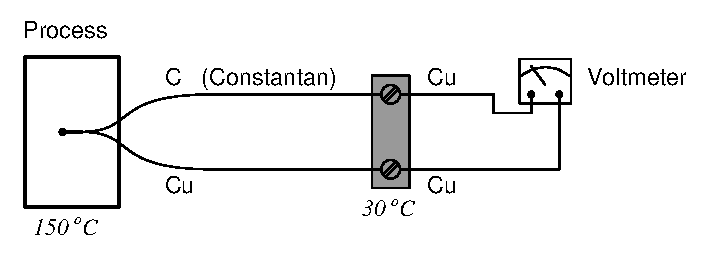
\includegraphics[width=15.5cm]{i00375x01.eps}$$

$$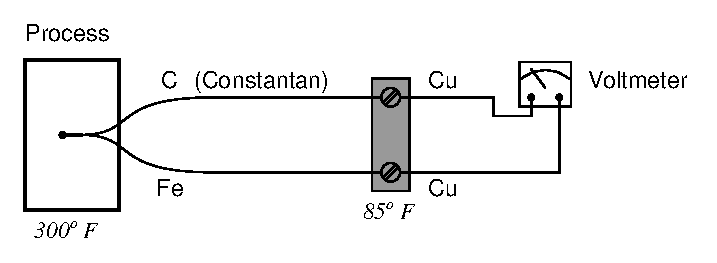
\includegraphics[width=15.5cm]{i00375x02.eps}$$

\underbar{file i00375}
%(END_QUESTION)





%(BEGIN_ANSWER)

Hint: for å løse oppgaven må du slå opp hvilken standard termoelementtype hver skjøt mellom ulike metaller tilsvarer. Referansematerialet oppgir hvilket metall som er positivt og hvilket som er negativt.

$$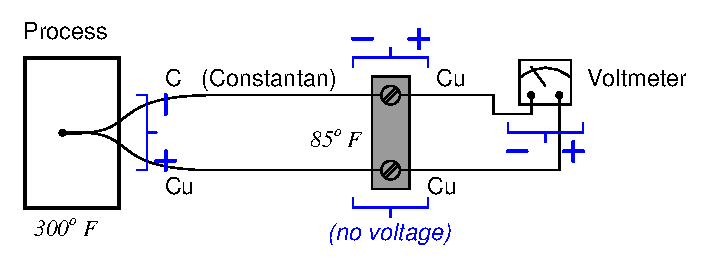
\includegraphics[width=15.5cm]{i00375x03.eps}$$

$$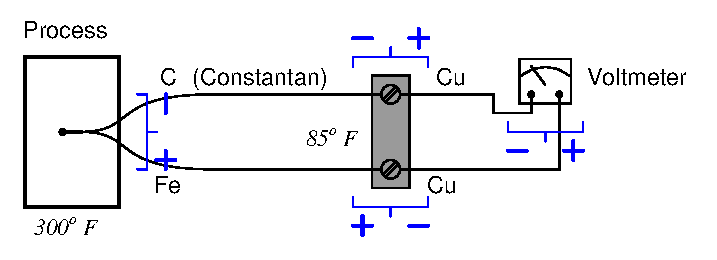
\includegraphics[width=15.5cm]{i00375x04.eps}$$


%(END_ANSWER)





%(BEGIN_NOTES)

Polaritet for Constantan-Kobber-skjøter finnes ved å slå opp type T-termoelementer, som består av nettopp disse metallene. I type T er Kobber positiv (+) og Constantan negativ ($-$). Voltmeterets polaritet bestemmes med Kirchhoffs spenningslov: finn hvilken kobber-constantan-skjøt som lager størst spenning (den varmeste), og sett polaritet deretter.

Polariteten for jern-constantan-skjøten fås ved type J-tabell. Polariteten for kobber-constantan fås ved type T-tabell. Polariteten for jern-kobber kan bestemmes eksperimentelt (jern = + ; kobber = -).

%INDEX% Measurement, temperature: thermocouple

%(END_NOTES)
